\chapter{Mobile Networks}
The mobile telephones were at first introduced in the 60s, but were not so popular and required an
operator to connect the calls. Ever since, the technology has swiftly evolved, and now we have
smartphones, which are able to do many other things outside voice calls, and today there are even
more mobile phones than people in the world.\\ 
All those device are connected trough Mobile Networks, which allow radio user terminals , named User
Equipment(UE) or Mobile Stations(MS), to connect to global networks infrastructure, like the
Internet. A mobile network is divided into two parts: the \textbf{Radio Access Network}(RAN), which
is The part of the network that connects the UE to the core network, and the \textbf{Core
Network}(CN) itself, which is the part of the network that connects the RAN to the global network
infrastructure.\\
\begin{figure}[h]
  \centering
  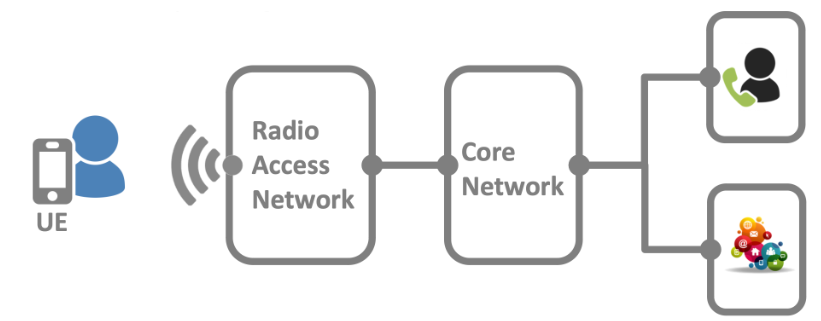
\includegraphics[width=0.5\textwidth]{img/wireless/mobile network overview.png}
  \caption{The overview of a mobile network}
  \label{fig:mobile-network}
\end{figure}
In the 2G and 3G technologies, the CN that provided access to the telephone service is based on
circuit-switched technology, which means that the connection between the two users is established
before the communication starts, and a separate core network is based on packet-switched technology,
to provide internet access. This was reverted after the 4G technology, in which the CN is based on
packet-switched technology to provide both telephone and internet services.\\
The main architectural elements of RAN are Base Transceiver Stations (BTS or BS) that
connect to UEs through a radio interface. For the newers technologies, like 4G and 5G, the BTS are
connected directly to the CN, but for the older ones, like 2G and 3G, the BTS are connected to an
additional radio controller placed between the BTS and the CN.\\
\begin{figure}[h]
  \centering
  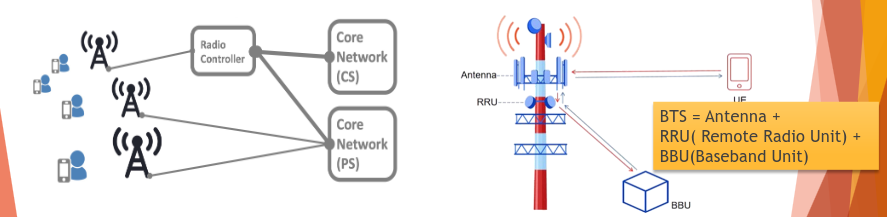
\includegraphics[width=0.7\textwidth]{img/wireless/mobile base stations.png}
  \caption{An overview of the placement of the base stations}
  \label{fig:mobile-architecture}
\end{figure}
\begin{section}{Cellular network Cells}
  Nowadays, the BSs are placed practically everywhere, because the SNR scales quadratically with the
  distance, to provide connectivity at any position, and the UEs can connect to the most convenient
  BS, which is usually the closest one. The area covered by a BS is called a \textbf{cell}.\\
  Historically, the cells share is considered \textit{hexagonal}, but in reality they are not, because
  signals do not propagate in a straight line, and the cells are usually irregularly shaped. The
  hexagonal approximation is used to simplify the calculations.
  \begin{subsection}{Frequency reuse}
    Radio waves are a limited resource, and the same frequency cannot be exclusively dedicated to a
    channel in a cell. But if the same frequency is reused, which is the basic idea, it generate
    interference, which is not ideal, so the cells are divided into \textbf{clusters}, which allows
    to reuse frequencies provided that the interference is limited and constrained. Each cluster
    have a pattern, that can be repeated for each cluster without generating too much interference.
    After all, if we consider a individual cell to have homogeneous traffic, and $k$ frequencies
    have to be assigned between a group of cells, you can notice that this problem is reducible to a
    \textbf{graph coloring problem}, which is NP-hard.
  \end{subsection}

  \begin{subsubsection}{Cell sizes}
    There are actually different sized of cells, which are used to provide different coverage and
    capacity. 
    \begin{itemize}
      \item \textbf{Macrocells} are the largest cells, and are used to provide coverage in rural
        areas, where the density of users is low.
      \item \textbf{Microcells} are used to provide coverage in urban areas, where the density of
        users is high, and the cells are smaller to provide more capacity.
      \item \textbf{Picocells} are used to provide coverage in buildings, like offices or shopping
        malls, where the density of users is very high.
      \item \textbf{Femtocells} are used to provide coverage in homes, where the density of users
        issues very high.
    \end{itemize}
    \begin{figure}[h]
      \centering
      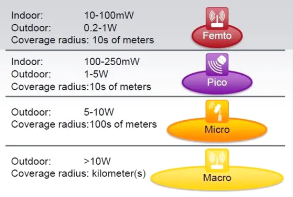
\includegraphics[width=0.4\textwidth]{img/wireless/cell sizes.png}
      \caption{The different sizes of cells}
      \label{fig:cell-sizes}
    \end{figure}
  \end{subsubsection}

  \begin{subsection}{Mobility Management}
    Users are not static in space, but they are able to move freely in the cell, and between cells.
    The network must thus be able to manage the mobility of the users, and to do so it uses a
    mechanism called \textbf{Handover}, tracking the user's position(in term of cell) and changing
    the network to adapt routing and commands to with the connection to the new cell.\\
    \begin{figure}[h]
      \centering
      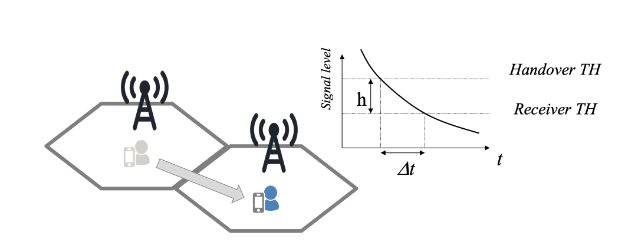
\includegraphics[width=0.5\textwidth]{img/wireless/mobile handover.png}
      \caption{An overview of the handover process}
      \label{fig:handover}
    \end{figure}
    The network is constantly monitored to check the signal strength and the quality of each
    neighboring cell, in respect to the MS, which measurements are sent to the BS every 480ms(at
    least for GMS). When the signal strength of the current cell is drops below a certain
    \textbf{threshold}, or becomes lower than the signal strength of a neighboring cell, the
    handover process is started by sending an \textbf{handover request} to the MS via the BTS which
    is serving the MS. While the MS is preparing, the network sends an \textit{Immediate Assignment}
    message to the MS, which contains the frequency and the time slot to use to connect to the new
    cell, and will be followed by the MS. Once the MS is successfully handed over to the new cell,
    data and voice traffic are transferred to the new cell, and after it is completed by a
    \textit{Handover confirmation} message, the old connection is released.\\
    If the handover process results in a change in the Base Station Controller (BSC) or Mobile
    Switching Center (MSC), new connections are established with the new controllers.The old BSC and
    MSC release resources associated with the call and update their databases with the MS’s new
    location information.
  \end{subsection}

  \begin{subsection}{Mobile Updates}
    The users can still move but not want an handover to be performed, for example when the user is
    moving very fast. In this case, the network is then divided in Location Areas(LAs), which are
    a set of cells. The MS sends a \textit{Location Update Request} to the network, and if the MS 
    change the LA, the position database is updated.\\ 
    This procedure is also very useful to know where the device is, and the process to find out
    exactly where the device is called \textbf{paging}. All base stations in LA broadcast a paging 
    message with the ID of the called user. When the mobile terminal replies, the network knows
    where the device is, and can establish a connection.
    \begin{figure}[h]
      \centering
      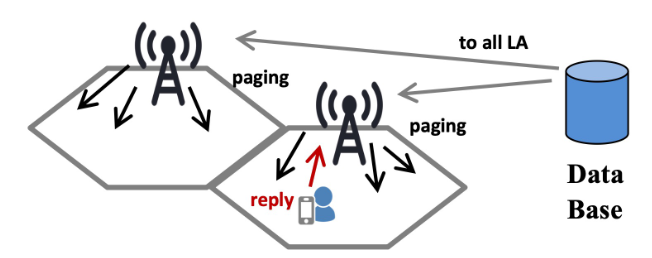
\includegraphics[width=0.5\textwidth]{img/wireless/mobile paging.png}
      \caption{An overview of the paging process}
      \label{fig:paging}
    \end{figure}
    \begin{subsubsection}{Paging vs Location update}
      The larger are the LA, the less frequent are the location updates, but the more frequent are 
      the paging messages. The smaller are the LA, the more frequent are the location updates, but
      the less frequent are the paging messages. The size of the LA is a trade-off between the
      frequency of the location updates and the frequency of the paging messages.
      This also depends on the mobility of the users, and the arrival frequency of the calls.
    \end{subsubsection}
  \end{subsection}
\end{section}

\begin{section}{Signalling}
  Signalling, in mobile networks, is in charge of establishing, maintaining, and terminating a
  service, assigning resources or modify them.
  In a classic telephone service, the signalling is in charge of routing and setting up circuits for
  phones, while in a mobile(IP) network, the signalling is used to set up media sessions.\\
  The basic service provided by signalling is the Basic Call that is used to set up a telephone
  call. Signalling hash two main components: the user signalling and the network signalling.
  \begin{paragraph}{User signalling}
    The user signalling is used to allow communication between user terminals and the network, and
    in particular to:
    \begin{itemize}
      \item ask for a service
      \item indicate the called party
    \end{itemize}
    The required information about the call status are provided by the network.
  \end{paragraph}
  \begin{paragraph}{Network signalling}
    The network signalling is used to allow communication between switching stations, and in
    particular to:
    \begin{itemize}
      \item route calls among the available paths
      \item allocate resources
      \item management operations
    \end{itemize}
    It is also used for providing supplementary services like special numbers(like 911), calling
    party notifications, mobility management, and so on.
  \end{paragraph}
  \begin{figure}[h]
    \centering
    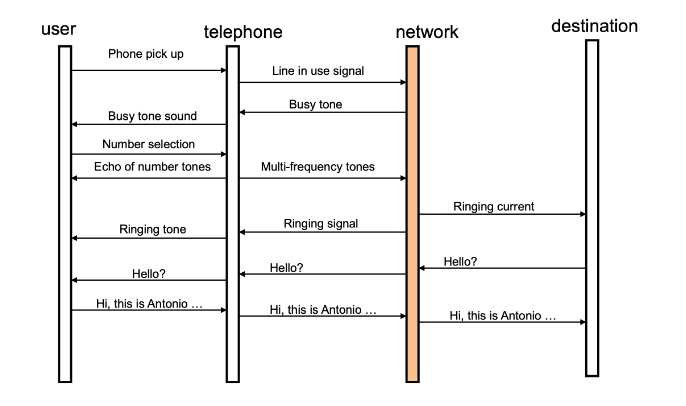
\includegraphics[width=0.6\textwidth]{img/wireless/signalling.png}
    \caption{An overview of the signalling process for a simple call}
    \label{fig:signalling}
  \end{figure}
  \begin{subsection}{Digital user signalling}
    We are now in a digital era, and the user signalling is now digital. ISDN, which stands for
    Integrated Services Digital Network, is a set of communication standards for simultaneous
    digital transmission of voice, video, data, and other network services over the traditional
    circuits of the public switched telephone network. Digital interfaces works in
    a rather different fashion, because the information is sent in digital messages transmitted over
    L2 frames in the D channel of the ISDN interface. The set of protocols for user signalling
    defines the DSS1 signalling system, which are transported directly into LDAP frames.

    \begin{figure}[h]
      \centering
      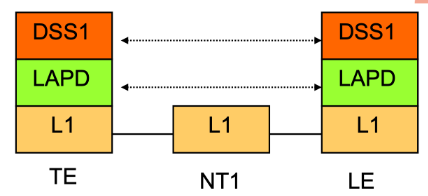
\includegraphics[width=0.4\textwidth]{img/wireless/digital user signalling.png}
      \caption{An overview of the digital signalling process}
      \label{fig:digital-signalling}
    \end{figure}

    \begin{figure}[h]
      \centering
      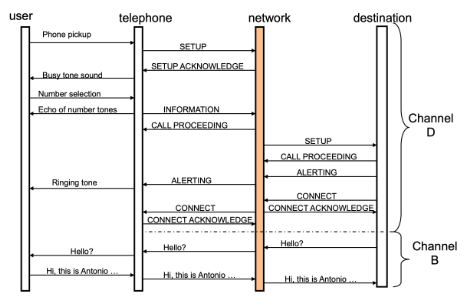
\includegraphics[width=0.5\textwidth]{img/wireless/digital user signalling exhange.png}
      \caption{The exchange of figure \ref{fig:signalling} in digital signalling}
      \label{fig:digital-signalling-2}
    \end{figure}
  \end{subsection}
  
  \begin{subsection}{Network signalling}
    Network signalling is a old standard, but still used today. The,kind of, modern signalling stack
    is called \textbf{SS7}, which stands for Signalling System 7, and is a set of telephony
    signalling protocols used for telephony, and which evolved to support all the services of modern
    fixed and mobile networks.\\
    The signalling is performed out-of-band, meaning that the signalling messages are transmitted
    over a separate network, and not over the same network used for the voice calls, and performed
    via packet switching.\\
    SS7 defines different kind of nodes:
    \begin{itemize}
      \item \textbf{Service Switching Points(SSP)} are the nodes that switch the calls and are
        responsible for the call control. They convert global titles digits(ie. phone numbers) into
        ss7 signalling messages.
      \item \textbf{Service Control Points(SCP)} are the nodes that provide application access to
        the network, and are responsible for the service logic.
      \item \textbf{Signal Transfer Points(STP)} are the nodes that route the messages between the
        SSPs and SCPs, and are responsible for the routing of the messages.
    \end{itemize}

    \begin{figure}[h]
      \centering
      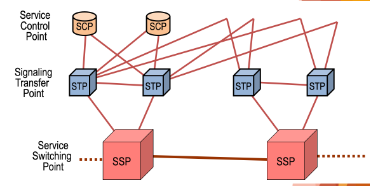
\includegraphics[width=0.5\textwidth]{img/wireless/ss7 architecture.png}
      \caption{An overview of the SS7 architecture}
      \label{fig:ss7}
    \end{figure}

    For the datagram packet switched network, The lower part of the SS7 protocol stack includes:
    \begin{itemize}
      \item Physical layer(MTP-1) defines the physical and electrical characteristics of the
        signalling links of the SS7 network, Signalling links utilise DS–0 channels and carry raw
        signalling data at a rate of 56 kbps or 64 kbps.
      \item Data link layer(MTP-2) provides link-layer functionality, in particular reliability
        and error detection.
      \item Network layer(MTP-3) provides routing functionality, and ensures that messages can be
        delivered between signalling points across the SS7 network regardless of whether they are
        directly connected. It also provides capabilities like node addressing, routing, alternate
        routing, and congestion control.
    \end{itemize}

    \begin{figure}[h]
      \centering
      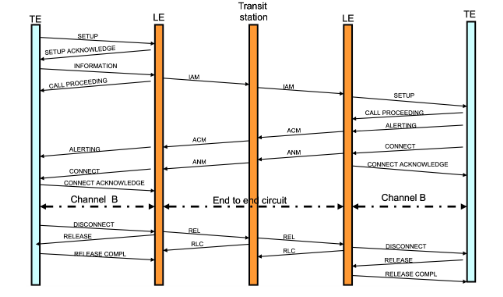
\includegraphics[width=0.5\textwidth]{img/wireless/ss7 digital call.png}
      \caption{The same call of figure \ref{fig:signalling} by the ss7 point of view}
      \label{fig:ss7-call}
    \end{figure}
    \begin{subsubsection}{Security in ss7}
      SS7 was designed in an era when security concerns were not considered. Every node in the SS7
      is trusted, because no authentication is performed, and the messages are not encrypted. 
      A lot of nasty attack can be performed, like:
      \begin{itemize}
        \item \textbf{Location tracking} by sending a location request to the network, and the
          network will reply with the location of the user.
        \item \textbf{SMS interception} by sending a SMS request to the network, and the network will
          reply with the SMS.
        \item \textbf{Call interception} by sending a call request to the network, and the network
          will reply with the call.
        \item \textbf{Denial of service} by sending a lot of messages to the network, and the network
          will be overloaded.
        \item \textbf{Fraud} by sending a call request to the network, and the network will reply
          with the call, but the call will be charged to the victim.
      \end{itemize}
      All those attacks are still possible today.
      \begin{figure}[h]
        \centering
        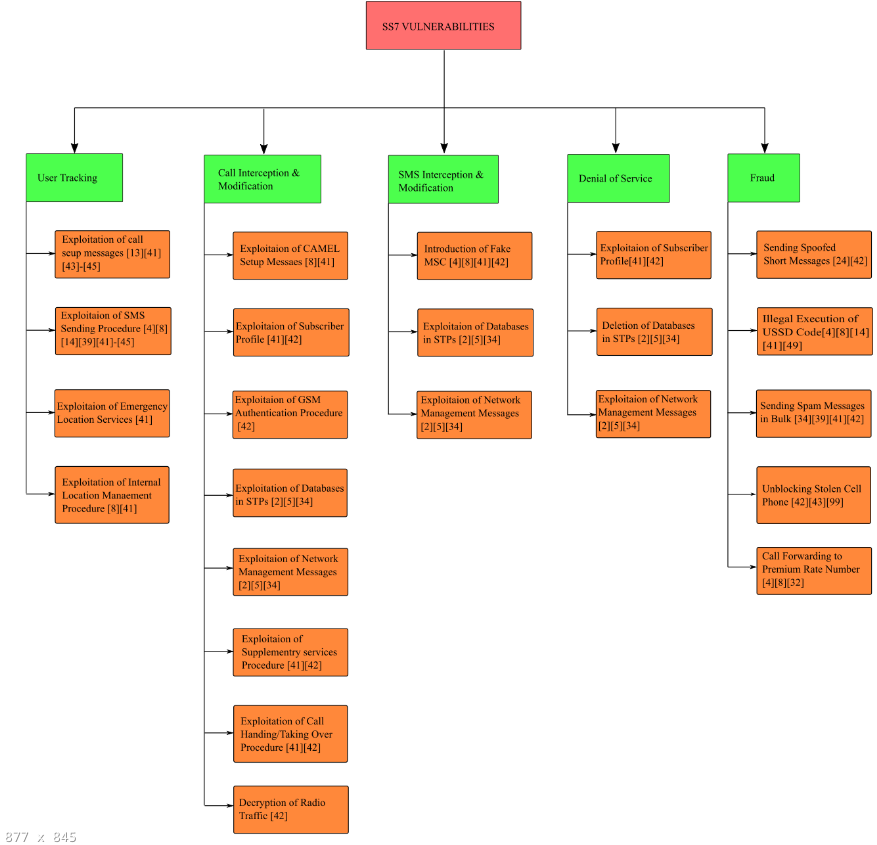
\includegraphics[width=0.5\textwidth]{img/wireless/ss7 attacks.png}
        \caption{An overview of the SS7 attack}
        \label{fig:ss7-attack}
      \end{figure}
    \end{subsubsection}
  \end{subsection}
\end{section}

\begin{section}{GSM network}
  The first network architecture of GSM was for circuit switched (CS) services only, and telephone
  service in particular. It was mainly divided into three parts( the UE, the RAN, and the CN), and 
  the CN was divided into three parts: 
  \begin{itemize}
    \item \textbf{Mobile Switching Center(MSC)} is the equivalent of a telephone station for the
      mobile network and includes all control and signalling functions for managing calls and
      mobility
    \item \textbf{Visitor Location Register(VLR)} is a database that contains information about all
      the mobile terminals currently located in the area controlled by the MSC
    \item \textbf{Home Location Register(HLR)} is a database that contains information about all the
      mobile terminals that are registered in the network. It also includes an AuC (Authentication
      Centre) for security procedures
    \item \textbf{Gateway MSC(GMSC)} is the MSC connecting the mobile network to the external
      telephone networks (PSTN) and that implements all signalling interworking functions
  \end{itemize}
  while the RAN was divided into two parts:
  \begin{itemize}
    \item \textbf{Base Transceiver Station(BTS)} is the GSM base station that manages physical layer
      connections with the UEs and the BSC and executes resource allocation commands received by the
      BSC
    \item \textbf{Base Station Controller(BSC)} is the GSM controller that implements higher layer
      protocols and manages all transmission resources of the connected BTSs
  \end{itemize}
  the UM radio intermace of GSM is based on the TDMA technology, but because it still uses the
  classical telephone transport network, the achievable data rate is limited to 65 kbps, and 2048
  Mbps while using E1 links.\\

  \begin{figure}[h]
    \centering
    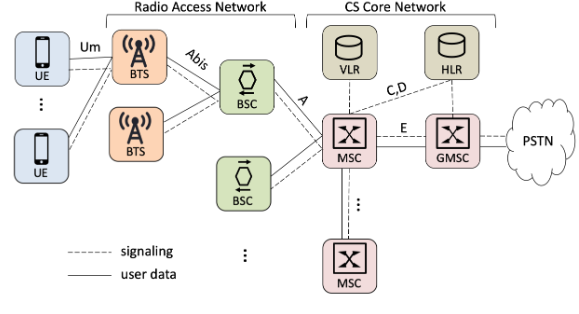
\includegraphics[width=0.5\textwidth]{img/wireless/gsm network.png}
    \caption{An overview of the GSM architecture}
    \label{fig:gsm-architecture}
  \end{figure}
  Of course, signalling is not very efficient, so schanging the infrastructure to a packet-switched
  network is a good idea. The first step was to introduce the GPRS, which stands for General Packet
  Radio Service, which is a packet-switched technology that allows the transmission of data over the
  GSM network. The GPRS network adds some new elements to the GSM network:
  \begin{itemize}
    \item \textbf{Serving GPRS Support Node(SGSN)} is an IP router which plays the same role as the
      MSC in the circuit- switched core, while also having additional functionalities for the
      management of the interfaces and protocols towards the BSS
    \item \textbf{Gateway GPRS Support Node(GGSN)}
  \end{itemize}
\end{section}

\begin{section}{UMTS networks}
  UMTS, or Universal Mobile Telecomunication System, focused on the introduction of better data
  services, by defining a new achitecture, separating the signalling protocols and procedures
  related to the radio access network and those related to the core network to allow future
  evolutions of the core network independent from the access network.\\

  Take a look at the figure \ref{fig:umts-architecture}, you can see that the radio part has been
  modified:
  \begin{itemize}
    \item \textbf{Node B} is the UMTS base station responsible for all functions required for
      sending and receiving data over the air interface( which is based on CDMA). Allocation
      commands received by the RNC. Is also responsible for the power control of all connections
    \item \textbf{Radio Network Controller(RNC)} is the main element of the UTRAN, responsible for
      controlling radio resources of all Node-Bs and mobility. 
  \end{itemize}

  \begin{figure}[h]
    \centering
    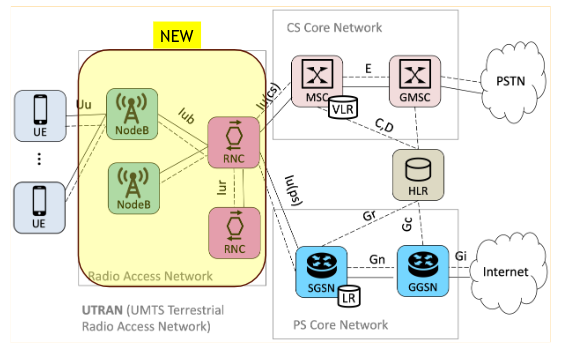
\includegraphics[width=0.5\textwidth]{img/wireless/umts architecture.png}
    \caption{An overview of the UMTS architecture}
    \label{fig:umts-architecture}
  \end{figure}
  The architecture was also modified in the core network, which changed the circuit-switched
  part even for voice calls. The switches became media gateways, which are ip based(VoIP), but
  signalling is still needed.\\
  \begin{figure}[h]
    \centering
    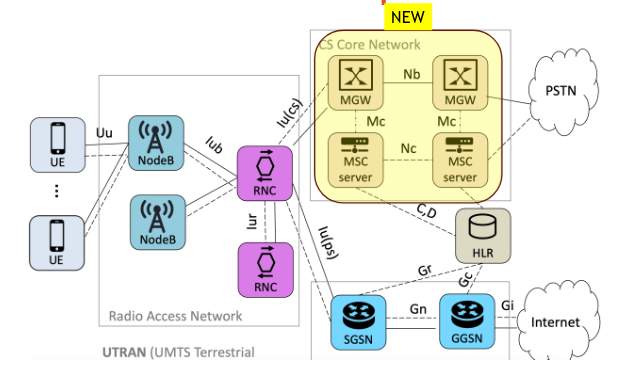
\includegraphics[width=0.5\textwidth]{img/wireless/umts 2.png}
    \caption{The changes in the core network of UMTS}
    \label{fig:umts-core}
  \end{figure}
  The result is that 2G and 3G networks are now fully integrated, and the same network can provide
  both voice and data services.\\

  \begin{subsection}{Implementational Details}
    In GMS, multiple access is based on FDM or TDM, with channels of 200 kHz, while are further 
    split into smaller channels of 45MHz, separating the uplink and downlink. A time slot is 577
    $\mu$s long, and each device can transmit for 8 time slots, or 4.615 ms.\\
    It implements frequency hopping to avoid interference, and power control to be power efficient.
    One of the main issue is synchronization, because of TDMA, because of the delay and the slot
    offsets. Signalling is also a problem, because of the need of a lot of messages to establish a
    call. Its still based on SS7, but because now the network is packet-switched, support for mobile
    signalling is added via a Mobile Application Part(MAP) protocol.\\
    \begin{figure}[h]
      \centering
      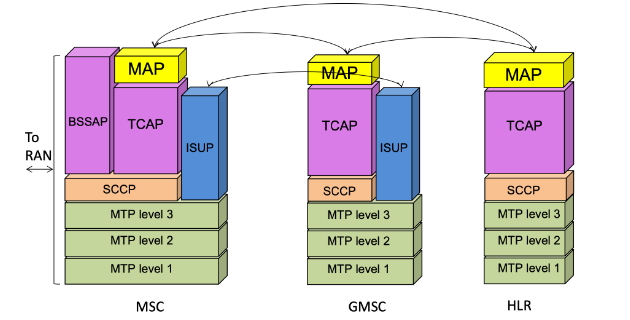
\includegraphics[width=0.5\textwidth]{img/wireless/mobile ss7.png}
      \caption{How MAP was added to the SS7 stack}
      \label{fig:mobile-ss7}
    \end{figure}
  \end{subsection}

\end{section}

\begin{section}{4g}
  In the 4th generation of mobile networks, everything is based on IP, even signalling, meaning that
  signalling is now performed over the same network used for the voice and data traffic. The
  architecture was simplified, being built from scratch, implementing a new "flat" architecture.
  The radio interface was also modified, and the new radio interface supports different bandwidths
  (from 1.25 to 20 MHz) and frequencies.

  \begin{figure}[h]
    \centering
    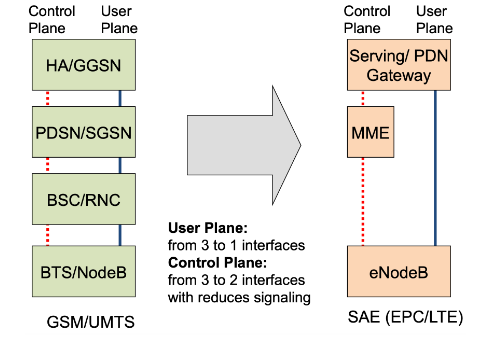
\includegraphics[width=0.5\textwidth]{img/wireless/4g evolution.png}
    \caption{The evolution of the mobile networks}
  \end{figure}
  \begin{subsection}{SAE}
  \end{subsection}

\end{section}

\begin{section}{GMS security}
  Historically, the only reason to have any kind of security in the mobile network was for
  subscriber authentication, for the sake of billing. The security was based on a Long-term secret
  key shared between the subscriber and the home network operator and checked via a
  challenge-response mechanism, and the secret was stored in the SIM card.\\
  GMS provides also means for confidentiality of communications and signalling over the wireless
  interface via encryption using encryption key shared between the subscriber and the visited
  network, also to support roaming, and means for anonymity of the subscriber.\\

  As you can recall, the GMS architecture is made up of three main parts: 
  \begin{itemize}
    \item \textbf{Mobile Station(MS)} is the mobile device(subscriber). It does all the user-side
      chypering, storing the secret key, and implementing the encryption algorithm. It is only
      hardware, so it still needs a SIM card to work.
    \item \textbf{Radio Access Network(RAN/BSS)} is the part of the network that connects the MS to
      the network. This part of the network implements the \textbf{encryption algorithms}, making
      all the communication secure from and to the MS. This means that only the wireless channel is
      encrypted.
    \item \textbf{Network and Switching Subsystem(NSS)} is the part of the network that connects the
      BSS to the network. They need to support authentication, storing all the keys are stored and
      managed by it. The Authentication Center(AuC) is the part of the NSS that is responsible for
      generationg the keys, which are stored in the Home Location Register(HLR).
  \end{itemize}

  \begin{subsection}{Sim}
    The SIM, or Subscriber Identity Module, is a smart card that stores network-specific information
    used to authenticate and identify subscribers on the network. It implements the cryptographic
    algorithms in hardware(not the most complicated ones, because they have to be cheap), and have
    some protected storage for the keys and personal information.\\
    It stores:
    \begin{itemize}
      \item \textbf{ICCID} is the unique identifier of the SIM card
      \item \textbf{IMSI} the international mobile subscriber identity, which is unique
      \item \textbf{$K_i$} is the secret key shared between the subscriber and the network, used for
        authentication
      \item Operator-specific emergency number
      \item some other data
    \end{itemize}

    \begin{figure}[h]
      \centering
      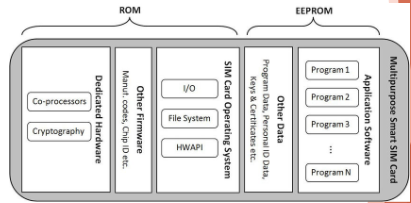
\includegraphics[width=0.7\textwidth]{img/wireless/sim.png}
      \caption{The SIM card}
    \end{figure}
  \end{subsection}
  
  \begin{subsection}{GSM Authentication}
    For authentication, the sim card is trusted, but not the phone itself. Becuase they are issued
    by the operator, they are trusted by the phone, but not the network it is eventually roaming
    into. The channel is never trusterd, but the core operator core network is(no encryption is
    required there).\\
    \begin{boxH}
      Thus, authenticate the SIM – and trust the operator network
    \end{boxH}
    Authentication is a one-way challenge-response protocol, based on the secret key $K_i$ stored in
    the SIM card.\\
    The entity authentication allows to authenticate the subscriber and to defend against
    unauthorised users at the same time. During authentication, 3 components are used:
    \begin{itemize}
      \item \textbf{Home Network Authentication Center(HNAC)} provides parameters for authentication
        and encryption functions of the original subscriber. Stores all subscriber identities and
        keys
      \item \textbf{Home Network HLR} provides MSC/VLR with authentication triplets (RAND, SRES, Kc)
        Handles MS location for the original subscribe
      \item \textbf{Visited Network Authentication Center(VNAC)} Stores generated triplets when a
        subscriber is not in the home network
    \end{itemize}
    The algorithms were never discosed, in fact each operator has its own algorithm, which never
    was used but still. The most common ones were A3, A5, and A8.\\
    A3 is the authentication algorithm, A8 is the session key generation algorithm, which used a
    PRNG. The authetication happened using a nonce signed via the secret key.
    \begin{boxH}
      Security procedures are logically managed by SIM card and AuC.
    \end{boxH}
    The parameters of the authentication are:
    \begin{itemize}
      \item \textbf{RAND} is a 128-bit random number generated by the AuC and then sent to the MSC
      \item \textbf{SRES} is the signed response, generated by the SIM card
      \item \textbf{$K_i$} is the authentication key (the secret) of 128 bits stored in the AuC and
        in the SIM
      \item \textbf{A3} is the algorithm for the authentication stored in the AuC and the SIM
      \item \textbf{A8} is the algorithm for the session key generation stored in the AuC and the
        SIM
    \end{itemize}
    The authentication process is shown in figure \ref{fig:authentication} and is as follows:
    \begin{enumerate}
      \item The MS sends its IMSI to the VLR, which forwards it to the HLR
      \item The HLR generate the challenge based on the triplet (RAND, SRES, Kc) and sends it to the
        VLR. (RAND is generated by the AuC)
      \item The VLR sends the RAND to the MSC
      \item The MS knows both the RAND and the Kc, and can calculate the SRES and send it to the VLR
      \item If the SRES is the same as the one generated by the HLR, the MS is authenticated
    \end{enumerate}

    \begin{figure}[h]
      \centering
      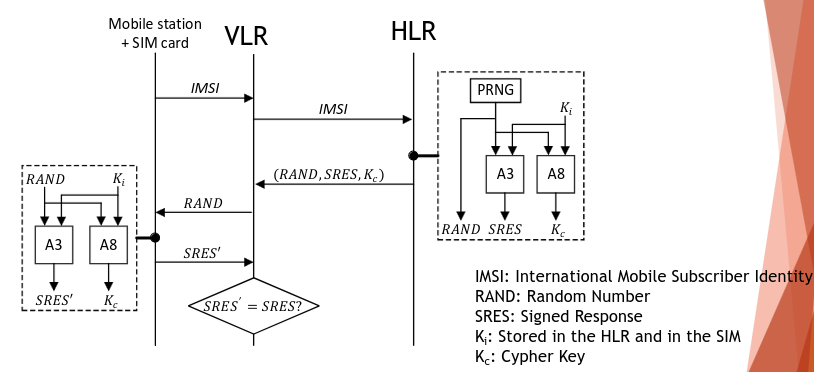
\includegraphics[width=0.7\textwidth]{img/wireless/gms auth.png}
      \caption{The authentication process}
      \label{fig:authentication}
    \end{figure}
    This schema is based on the strength of the cryptographic algorithms, if those are broken, the
    whole system is broken, and a attacker can decrypt everything. This was easily doable because
    the same parameters were used for more than one encryption schema. Furthermore, no base station
    authentication is performed, so mitm attacks are possible.\\
    The encryption of the communication is performed by the A5 algorithm, which is a stream cipher
    that encrypts the data in the radio interface. The core network traffic is not encrypted for
    legal reasons.
    \begin{subsubsection}{VLR Changes and mobility}
      When a user has moved to a new VLR, the new VLR will normally establish the subscriber’s
      identity by requesting the IMSI from the old VLR.\\
       The old VLR transfers, together with the IMSI, any unused triplets to the new VLR. This
       speeds up the authentication procedure because the new VLR can only send a request for
       triplets to the subscriber’s HLR/AuC after it has learned of the “real” identity of the
       subscriber which is through this request to the old VLR.

    \end{subsubsection}

   \end{subsection}

   \begin{subsection}{A3 and A8}
     \begin{subsubsection}{A3}
       The A3 is lighweigth encryption algoritm, which takes in input:
       \begin{itemize}
         \item \textbf{RAND} is a 128-bit random number generated by the AuC and then sent to the MSC
         \item \textbf{$K_i$} is the authentication key (the secret) of 128 bits stored in the AuC and
           in the SIM
       \end{itemize}
       It runs in under 500ms.
       \begin{figure}[h]
         \centering
         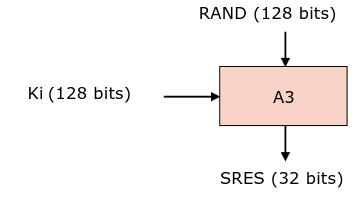
\includegraphics[width=0.4\textwidth]{img/wireless/a3.png}
         \caption{The A3 algorithm}
       \end{figure}
     \end{subsubsection}
     \begin{subsubsection}{A8}
       The A8 is the session key generation algorithm, which used a PRNG. It takes in input:
       \begin{itemize}
         \item \textbf{RAND} is a 128-bit random number generated by the AuC and then sent to the MSC
         \item \textbf{$K_i$} is the authentication key (the secret) of 128 bits stored in the AuC and
           in the SIM
       \end{itemize}
       It was secure because of Security by obscurity, but it was broken easily because one leaked
       it was really not that secure. 
       \begin{figure}[h]
         \centering
         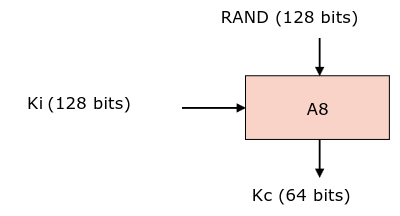
\includegraphics[width=0.4\textwidth]{img/wireless/a8.png}
         \caption{The A8 algorithm}
       \end{figure}
      \end{subsubsection}
      \begin{subsubsection}{COMP128}
        In most GSM networks, A3 and A8 are derived from the algorithm COMP128. It is a keyed hash
        function which takes in input:
        \begin{itemize}
          \item \textbf{RAND} is a 128-bit random number generated by the AuC and then sent to the MSC
          \item \textbf{$K_i$} is the authentication key (the secret) of 128 bits stored in the AuC and
            in the SIM
        \end{itemize}
        and outputs a 12 bytes hash(32 bits are the SRES, 64 bits are the Kc). 

        \begin{figure}[h]
          \centering
          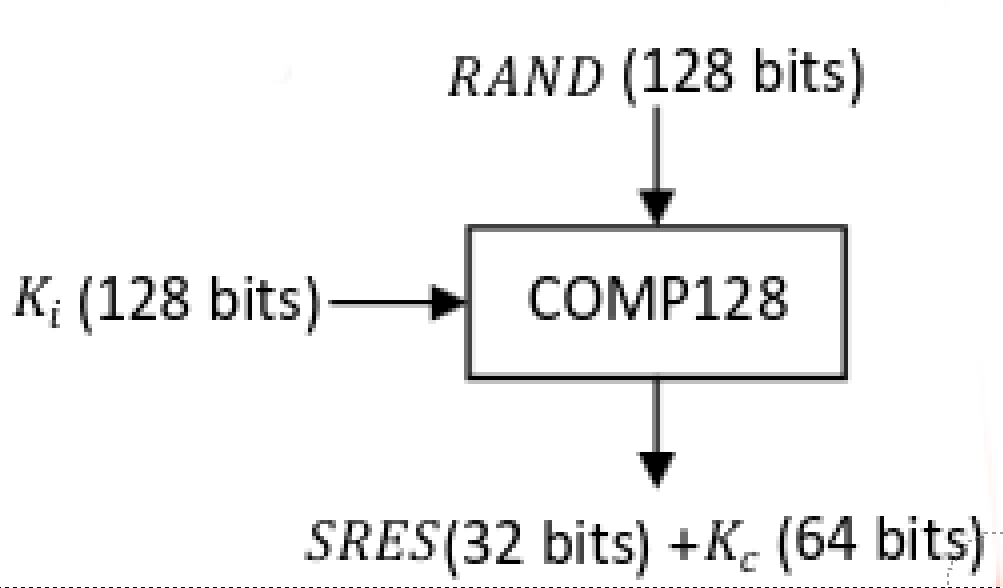
\includegraphics[width=0.4\textwidth]{img/wireless/comp128.png}
          \caption{The COMP128 algorithm}
        \end{figure}

        It works like this:
        \begin{enumerate}
          \item Loads Ki and RAND in a 32-byte vector X[]
          \item Ki is stored in X[0..15] and RAND is stored in X[16..31]
          \item Apply 8 iterative loops on X[]
            \begin{enumerate}
              \item Each iteration starts with a compression that follows the butterfly-structure
                \begin{itemize}
                  \item The compression consists of five levels of table lookups using T0[512], T1[256], T2[128], T3[64] and T4[32]
                  \item Each Ti contains only (8-i)-bit values
                \end{itemize}
              \item In all iterations except for the last, a permutation follows the compression
              \item Compression results in 32 4-bit values, which are then assembled into 16 bytes before the permutation is
                applied
              \item These 16 bytes are stored into X[16..31] and Ki is loaded into X[0..15] before a new iteration begins
            \end{enumerate}
          \item The resulting 128 bits after the eight iterations are further compressed to 12 bytes, which form the
            output of the algorithm
        \end{enumerate}

        In April of 1998, the Smartcard Developer Association along with 2 UC Berkeley researchers
        (Wagner/Goldberg) produced the first publicized attack on COMP128.
        It basically exploits a weakness in the second round of the compression function to generate
        a collision and recovering the Ki one byte at the time, and thus duplicate a sim card.
      \end{subsubsection}
    \end{subsection}

    \begin{subsection}{GMS Confidentiality}
      Confidentiality in GMS is provided by the A5 algorithm, whcih counts 7 version, all of which
      were initially kept secret, and published after some leaks. A5 is a stream cipher, because the
      voice communication is a stream of bits. The keystream is generated from a key of the client,
      which is salted with a frame number of 22 bits, generated a keystream of 114 bits. It was not
      used a true random number as salt because of "syncronization"(be the same for both the 
      transmitter and the receiver).
      \begin{figure}[h]
        \centering
        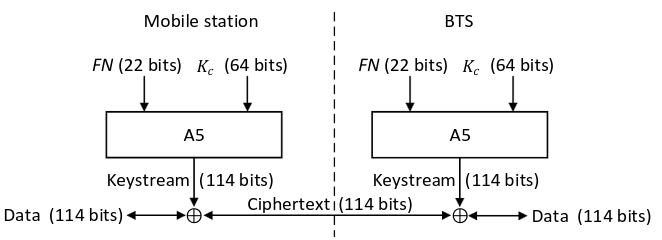
\includegraphics[width=0.6\textwidth]{img/wireless/a5.png}
        \caption{The A5 algorithm}
      \end{figure}
      \begin{subsubsection}{A5/1}
        The first implementation is aa simple combination of linear feedback shift register,
        respectively of 19, 22 and 23 bits. The middle bits decides which registers influences the
        result, enabling al least two registers at all times.

        \begin{figure}[H]
          \centering
          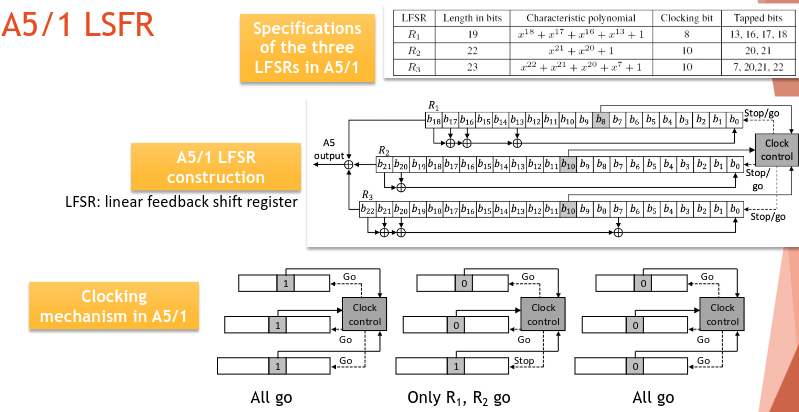
\includegraphics[width=0.6\textwidth]{img/wireless/a5-1.png}
          \caption{The A5/1 algorithm}
        \end{figure}

        \begin{figure}[H]
          \centering
          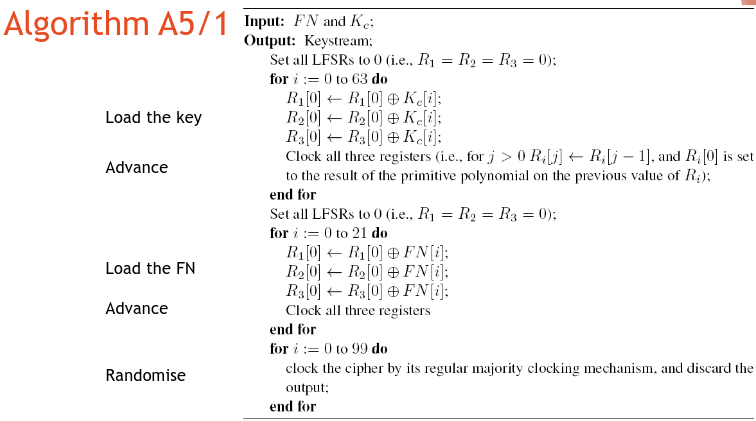
\includegraphics[width=0.6\textwidth]{img/wireless/a5-1 algorithm.png}
          \caption{The A5/1 algorithm}
        \end{figure}

      \end{subsubsection}
      \begin{subsubsection}{A5/2}
        A version used for export(for use in Eastern European states) is the second version. It is
        based opn a combination of 4 LFSR with irregular clocking and combined non linearly. It was
        missing the randomization phase, and was thus easily broken.

        \begin{figure}[H]
          \centering
          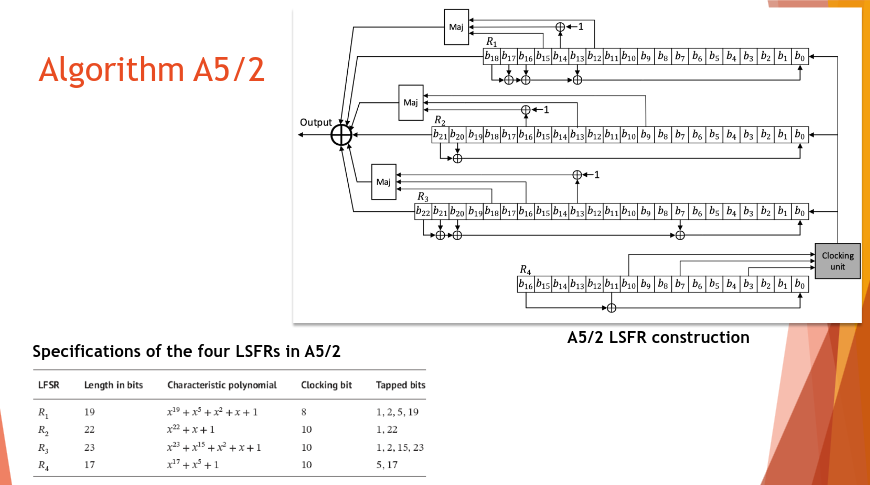
\includegraphics[width=0.6\textwidth]{img/wireless/a5-2.png}
          \caption{The A5/2 algorithm}
        \end{figure}
      \end{subsubsection}
    \end{subsection}
  \end{section}

  \begin{section}{GMS Anonymity}
    All communications are initiated by the MS that transmits its ID (IMSI) for activating the
    authentication procedure, and is transmitted in plaintext during authentication, or roaming,
    allwoing the tracking of the user. The solution is to allocate a temporary ID(TMSI) to the user
    each time a new VLR is visited. The TMSI is a 4-byte random number computed by the VLR and sent
    to the MS.

    \begin{figure}[h]
      \centering
      \includegraphics[width=0.6\textwidth]{img/wireless/tmsi.png}
      \caption{The TMSI allocation}
    \end{figure}

    \begin{subsection}{Stolen equipement}
      When mobile equipment is lost or stolen, its IMEI can be used for the detection of such
      equipment. The owner can report the loss of a cell phone to the network operator, who stores
      IMEI in the EIR (Equipment Identity Register) in a blacklist. The operator can optionally
      communicate the blacklist to a shared central EIR.
    \end{subsection}
  \end{section}

  \begin{section}{Attacks to GSM}
    All things that have previously mentioned can be attacked in GMS.
    \begin{itemize}
      \item Cryptanalysis attacks are possible against A3/A5/A8/COMP-128 algorithm
        \subitem This is possible trough a wireless interface
      \item Over-the-air interception using fake BTS (stingray), because the authentication is
        unilateral. MSI-catchers are used by law enforcement and intelligence agencies
      \item Only air interface transmission is encrypted
      \item Cyphering key Kc for encryption is only 54 bits long
      \item Key Ki recovery allows SIM cloning
      \item No message authentication and integrity protection is implemented
      \item DOS is possible by jamming a signal
    \end{itemize}
  \end{section}

  \begin{section}{UMTS security}
    A quick recap of the UMTS architecture(3G): it is based on the GMS architecture, extended with
    new elements to move all the services to a packet-switched network and to use WCDMA as the radio
    interface. 
    \begin{subsection}{UMTS Network Access Security}
      It is important to protect the radio access link, and even inside the core network.
      5 security features are required, as described by figure \ref{fig:umts-security}.
      \begin{figure}[h]
        \centering
        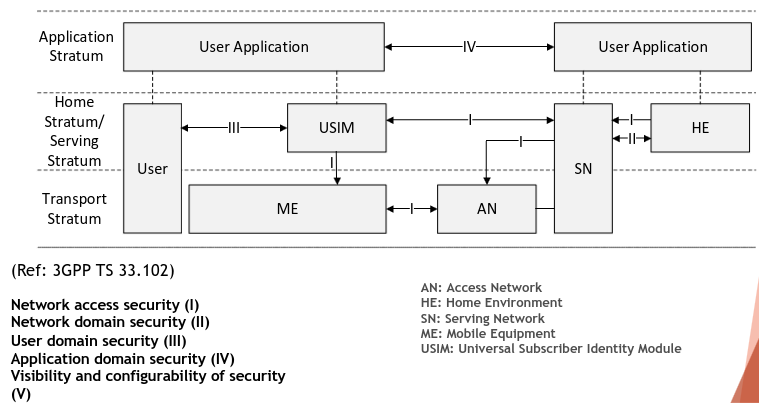
\includegraphics[width=0.6\textwidth]{img/wireless/umts security features.png}
        \caption{The UMTS security features}
        \label{fig:umts-security}
      \end{figure}
      Those 5 feaures are:
      \begin{itemize}
        \item \textbf{Network access security}: the set of security features that provide users with
          secure access to 3G services
        \item \textbf{Network domain security}: the set of security features that enable nodes in the
          provider domain to exchange signalling data securely
        \item \textbf{User domain security}: the set of security features that secure access to mobile
          stations
        \item \textbf{Application domain security}: the set of security features that enable
          applications in the user and the provider domain to exchange messages securely
        \item \textbf{Visibility and configurability}:  the set of features to inform the user
          whether a security feature is in operation or not and whether the use and provision of
          services should depend on the security feature
      \end{itemize}
      \begin{subsubsection}{Network Access Security}
        To provide secure access, a set of confidentiality, integrity, and authentication mechanisms
        are required. In particular it is introduced the concept of:
        \begin{itemize}
          \item Untracebility features, which are used to hide the identity of the user
          \item Network authentication, which was not present in GSM
          \item Confidentiality of signalling data
          \item Integrity checks
          \item Serialization of the packets to avoid replay attacks
          \item the ability to change the keys
        \end{itemize}

        The mechanism for authentication and key agreement requires the following cryptographic
        functions:
        \begin{itemize}
          \item f1: network authentication function
          \item f2: the user authentication function
          \item f3: cypher key derivation function
          \item f4: integrity key derivation function
          \item f5: anonymity key derivation function
        \end{itemize}
        For each of the algorithms, there is a general requirement that it shall be computationally
        infeasible to derive K from knowledge of input(s) and output. The algorithms are based on 
        a shared secret key still.

        \begin{figure}[h]
          \centering
          \includegraphics[width=0.5\textwidth]{img/wireless/umts authentication.png}
          \caption{The UMTS security}
        \end{figure}

        The network generates a sequence number and a nonce, and by wnowing the key, it is used to
        generate: 
        \begin{itemize}
          \item \textbf{MAC} is the message authentication code
          \item \textbf{XRES} is the expected response
          \item \textbf{CK} is the cyphering key
          \item \textbf{IK} is the integrity key
          \item \textbf{AK} is the anonymity key
        \end{itemize}
        Because all the parameters are derived from the same key, all those parameters are also
        authenticated.

        \begin{figure}[h]
          \centering
          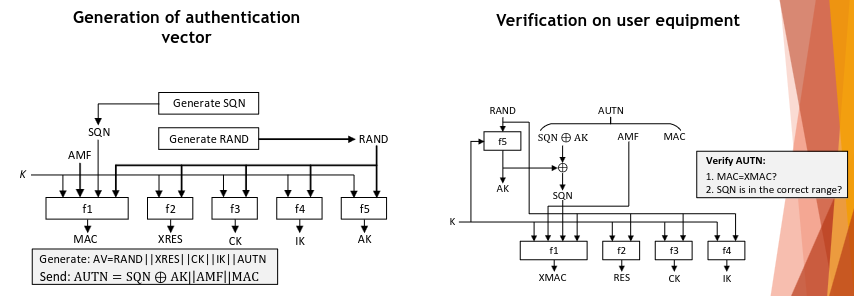
\includegraphics[width=0.5\textwidth]{img/wireless/umts authentication 2.png}
          \caption{The UMTS security in details}
        \end{figure}

      \end{subsubsection}

    \end{subsection}

  \end{section}
